%-----------------------------------------------------------------
%	PERFORMANCE
%	!TEX root = ./../main.tex
%-----------------------------------------------------------------
\section{Implementation of MPI}

\subsection{Setting up the system before working}

Before doing anything, we need to load the \inline{modules} of the compiler and libraries we have to use:
\begin{lstlisting}[language=bash]
module load gcc/6.1.0
module load openmpi/1.8.1
\end{lstlisting}

We need to compile the \inline{Makefile} to use TAU with MPI:
\begin{lstlisting}[language=bash]
cd tau-2.26
./configure -prefix=/home/master/ppM/ppM-1-10/my_TAU -mpi
export PATH=/home/master/ppM/ppM-1-10/my_TAU/x86_64/bin:$PATH
make install
\end{lstlisting}

We need to export the Makefile to the environment variable to be able to use TAU with MPI whilst compiling and running our C program, as well as the \inline{optCompInst} option:
\begin{lstlisting}[language=bash]
export TAU_MAKEFILE=/home/master/ppM/ppM-1-10/my_TAU/x86_64/lib/ Makefile.tau-mpi
export TAU_OPTIONS=-optCompInst
\end{lstlisting}

%-----------------------------------------------------------------
\subsection{Parallelisation with MPI}

To compile an MPI program we would usually compile the C code using \inline{mpicc}:
\begin{lstlisting}[language=bash]
mpicc -lm laplaceMPI.c -o compiledfile
\end{lstlisting}

However, to use TAU, we need to compile it using
\begin{lstlisting}[language=bash]
tau_cc.sh -lm laplaceMPI.c -o compiledfile
\end{lstlisting}

One of the main variables to consider when improving the performance of a code using MPI is the number of threads that we use. Specifying the exact number of threads to be used can be done easily when running the compiled  file. 

In the following snippet it is showed how to run the compiled code over a $1000 \times 1000$ matrix using $4$ threads.

\begin{lstlisting}[language=bash]
mpirun -np 4 compiledfile 1000
\end{lstlisting}

An important difference between the usage of OpenMP and MPI is that we specify the number of threads within the very code in the former, whereas we set the number of threads when executing the compiled file in the latter.

Using MPI we can improve greatly the performance of the code when used on sequential portions of the program, such as loops where each step is independent from the others.

\bigskip

In the proceeding section, we will explain our implementation of MPI to parallelise the code to solve 2D Laplace equation using Jacobi Iteration method.

%-----------------------------------------------------------------
\subsection{Basic parallel solution}

Suppose that we are going to use $N$ processes to solve the problem in a distributed way. Accordingly with the characteristics of the problem, each of these processes will have to carry on the computation over a portion of the matrix $A$, taking care for interchanging the necessary data and synchronising with other processes. The specific processes that will have to communicate will depend on how the data is partitioned among them.

The simplest partition of $A$ is shown in figure \ref{fig:a-matrix}. In this case, each process $P_{i}$ takes care of the computation of $m/N$ rows of $A$ and, in the general case ($0 < i < N-1$), it needs the last row of $P_{i-1}$ and the first of $P_{i+1}$.

\begin{figure}[H]
    \centering
    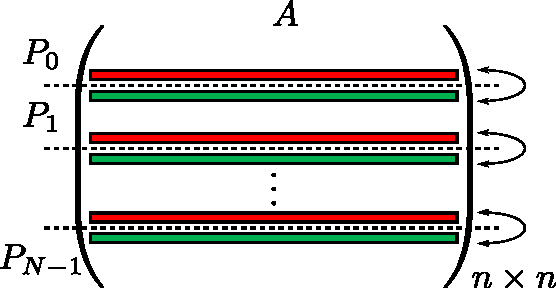
\includegraphics[width=0.45\textwidth]{images/a-matrix}
    \caption{Diagram of the partition of the matrix $A$}
    \label{fig:a-matrix}
\end{figure}

First of all, we need to define some variables in our C program that are needed for the MPI implementation, like \inline{rank}, \inline{size}, \inline{m}, \inline{ri}, \inline{rf}; and to initialize the MPI parallel region:

\begin{lstlisting}[firstnumber=52]
 // Variables needed for MPI
int rank, size;
\end{lstlisting}

We define the initial and final row of the subpartitions of the matrix as
\begin{align}
\begin{aligned}
    r_{i}[k] &= \frac{n}{N} \times \qty k \\
    r_{f}[k] &= \qty( \frac{n}{N} \times (k + 1) ) - 1 \\
\end{aligned}        
\end{align}
where $n$ is the dimension of the matrix, $N$ (or \inline{size}) is the amount of threads used, and $k = 0, \dots, N-1$ (or \inline{rank}) is the number of the working thread. Notice that Thread 0 will be used to make calculations as well as being the master thread to coordinate all computations. Notice that $n/N$ must be an integer.
 
\begin{lstlisting}[firstnumber=75]
// Initialisation of MPI parallel region
MPI_Init(&argc, &argv);
MPI_Comm_rank(MPI_COMM_WORLD, &rank);
MPI_Comm_size(MPI_COMM_WORLD, &size);
MPI_Status status;

// Define the partition of the matrix
int m = n/size;
int ri = rank * m, 
int rf = (rank+1) * m-1;
\end{lstlisting}

In the main loop of the program, we implement the basic parallel solution as described above. In the snippets below we can see excerpts of the script where MPI has been used. The rest of the program is almost identical to the standard implementation without MPI.

We can send and recieve messages from the different threads:
\begin{lstlisting}[firstnumber=96]
// Interchange of messages between consecutive rows
if ( rank > 0 ) {
	MPI_Send(&A[ri*n], n, MPI_FLOAT, rank-1, 1, MPI_COMM_WORLD);
	MPI_Recv(&A[(ri-1)*n], n, MPI_FLOAT, rank-1, 2, MPI_COMM_WORLD, &status);
}
if ( rank < size-1 ) {
	MPI_Send(&A[rf*n], n, MPI_FLOAT, rank+1, 2, MPI_COMM_WORLD);
	MPI_Recv(&A[(rf+1)*n], n, MPI_FLOAT, rank+1, 1, MPI_COMM_WORLD, &status);
}
\end{lstlisting}

The main part of the program, performing the Laplace step function using the implemented partition of the matrix $A$:
\begin{lstlisting}[firstnumber=106]
// Computation of the Laplace Step using MPI
if ( rank == 0 ) {
	for ( j = ri+1; j <= rf; j++ ) {
		for ( i = 1; i < n-1; i++ ) {
			temp[j*n+i] = stencil(A[j*n+i+1], A[j*n+i-1], A[(j-1)*n+i], A[(j+1)*n+i]);
			error = max_error( error, temp[j*n+i], A[j*n+i] );
		}
	}
}
if ( rank == (size-1) ) {
	for ( j = ri; j < rf; j++ ) {
		for ( i=1; i < n-1; i++ ) {
			temp[j*n+i] = stencil(A[j*n+i+1], A[j*n+i-1], A[(j-1)*n+i], A[(j+1)*n+i]);
			error = max_error( error, temp[j*n+i], A[j*n+i] );
		}
	}
}
if ( rank != 0 && rank != (size-1) ) {
	for ( j = ri; j <= rf; j++ ) {
		for ( i = 1; i < n-1; i++ ) {
			temp[j*n+i] = stencil(A[j*n+i+1], A[j*n+i-1], A[(j-1)*n+i], A[(j+1)*n+i]);
			error = max_error( error, temp[j*n+i], A[j*n+i] );
		}
	}
}
\end{lstlisting}

We send the partial errors of each thread to the master:
\begin{lstlisting}[firstnumber=132]
// Sending partial errors to the master and computing the maximum to find the global error
if ( rank != 0 ) {
		MPI_Send(&error, 1, MPI_FLOAT, 0, 3, MPI_COMM_WORLD);
} else {
	errors[0] =error;
	for (i = 1; i < size; i++ ) {
		MPI_Recv(&errors[i], 1, MPI_FLOAT, i, 3, MPI_COMM_WORLD, &status);
	}
}
global_error = maximum(errors, size);
\end{lstlisting}

The master calcualtes the global error using the partial errors previously sent:
\begin{lstlisting}[firstnumber=143]
// Sending back the resulting error
if ( rank == 0 ) {
	for(i = 1; i<size; i++ ) MPI_Send(&global_error, 1, MPI_FLOAT, i, 4, MPI_COMM_WORLD);
} else {
	MPI_Recv(&global_error, 1, MPI_FLOAT, 0, 4, MPI_COMM_WORLD, &status);
}
\end{lstlisting}

As usual, once we've finished the computations, we need to \emph{close} MPI.
\begin{lstlisting}[firstnumber=156]
MPI_Finalize();
\end{lstlisting}

As it can be seen, it is almost the same algorithm implemented in the provided \inline{lapFusion.c} code, just distributing the work and adding the data interchange among processes.